\documentclass[varwidth=10in]{standalone}
\usepackage{tikz-qtree}

\begin{document}

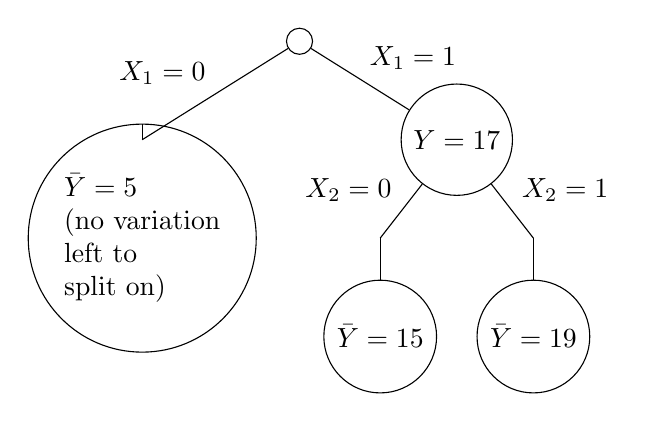
\begin{tikzpicture}[every tree node/.style={draw,circle},
   level distance=1.25cm,sibling distance=.5cm, 
   edge from parent path={(\tikzparentnode) -- (\tikzchildnode)}]

\Tree
    [.\node {};
      \edge node[auto=right] {$X_1 = 0$};  
      [\node[draw, align=left] {$\bar{Y}=5$\\(no variation \\left to\\ split on)};] 
      \edge node[auto=left] {$X_1 = 1$};  
 [.$Y=17$
      \edge node[auto=right] {$X_2 = 0$};  
[$\bar{Y}=15$ ]
      \edge node[auto=left] {$X_2 = 1$};  
[$\bar{Y}=19$ ]
    ]
]

\end{tikzpicture}


\end{document}